\section{Aim 3. Assess the impact of PRC2 dysregulation on the tissue-specificity of cancer driver genes.}

\subsection*{Rationale}

As explained by Haigis \emph{et al.} in \cite{Haigis2019}, substantial evidence has lead us to hypothesize that the potential for a gene to drive cancer is predominately determined by the preexisting state of the cell and tissue microenvironment.
This state is determined by the epigenetic structure established over the development of the tissue.
By regulating gene expression, epigenetics establishes the transcriptome and proteome, defining the cellular signaling network.
Only the disruption to specific genes and proteins are oncogenic within the context of this network, thus defining the tissue-specificity of cancer driver genes.

PRC2 is responsible for maintaining gene silencing by methylating H3K27, and its activity is often ascribed to maintaining a cell's functional identity \cite{Comet2016MaintainingCancer., Laugesen2019a}.
Because the genes comprising this protein complex are frequently mutated or dysregulated (via changes in expression or gene copy number) in cancer \cite{Wassef2017, Comet2016MaintainingCancer.}, we propose it as a system through which to investigate the impact of the epigenome on tissue-specificity of cancer drivers.
\textbf{We hypothesize that the dysregulation of PRC2 methylation alters the state of a cell, and consequently alters the oncogenic potential of cancer driver genes.}

For this study, we will use data from a cancer type with a large number of sequenced samples and a high frequency of PRC2 mutations.
From a cursory inspection of The Cancer Genome Atlas (Figure \ref{fig:num-samples-prc2}), we propose using ovarian, uterine, breast, or skin cancer, though we will also account for data from other large consortia (such as the Pan-Cancer Analysis of Whole Genomes).

\begin{figure}[ht]
\centering
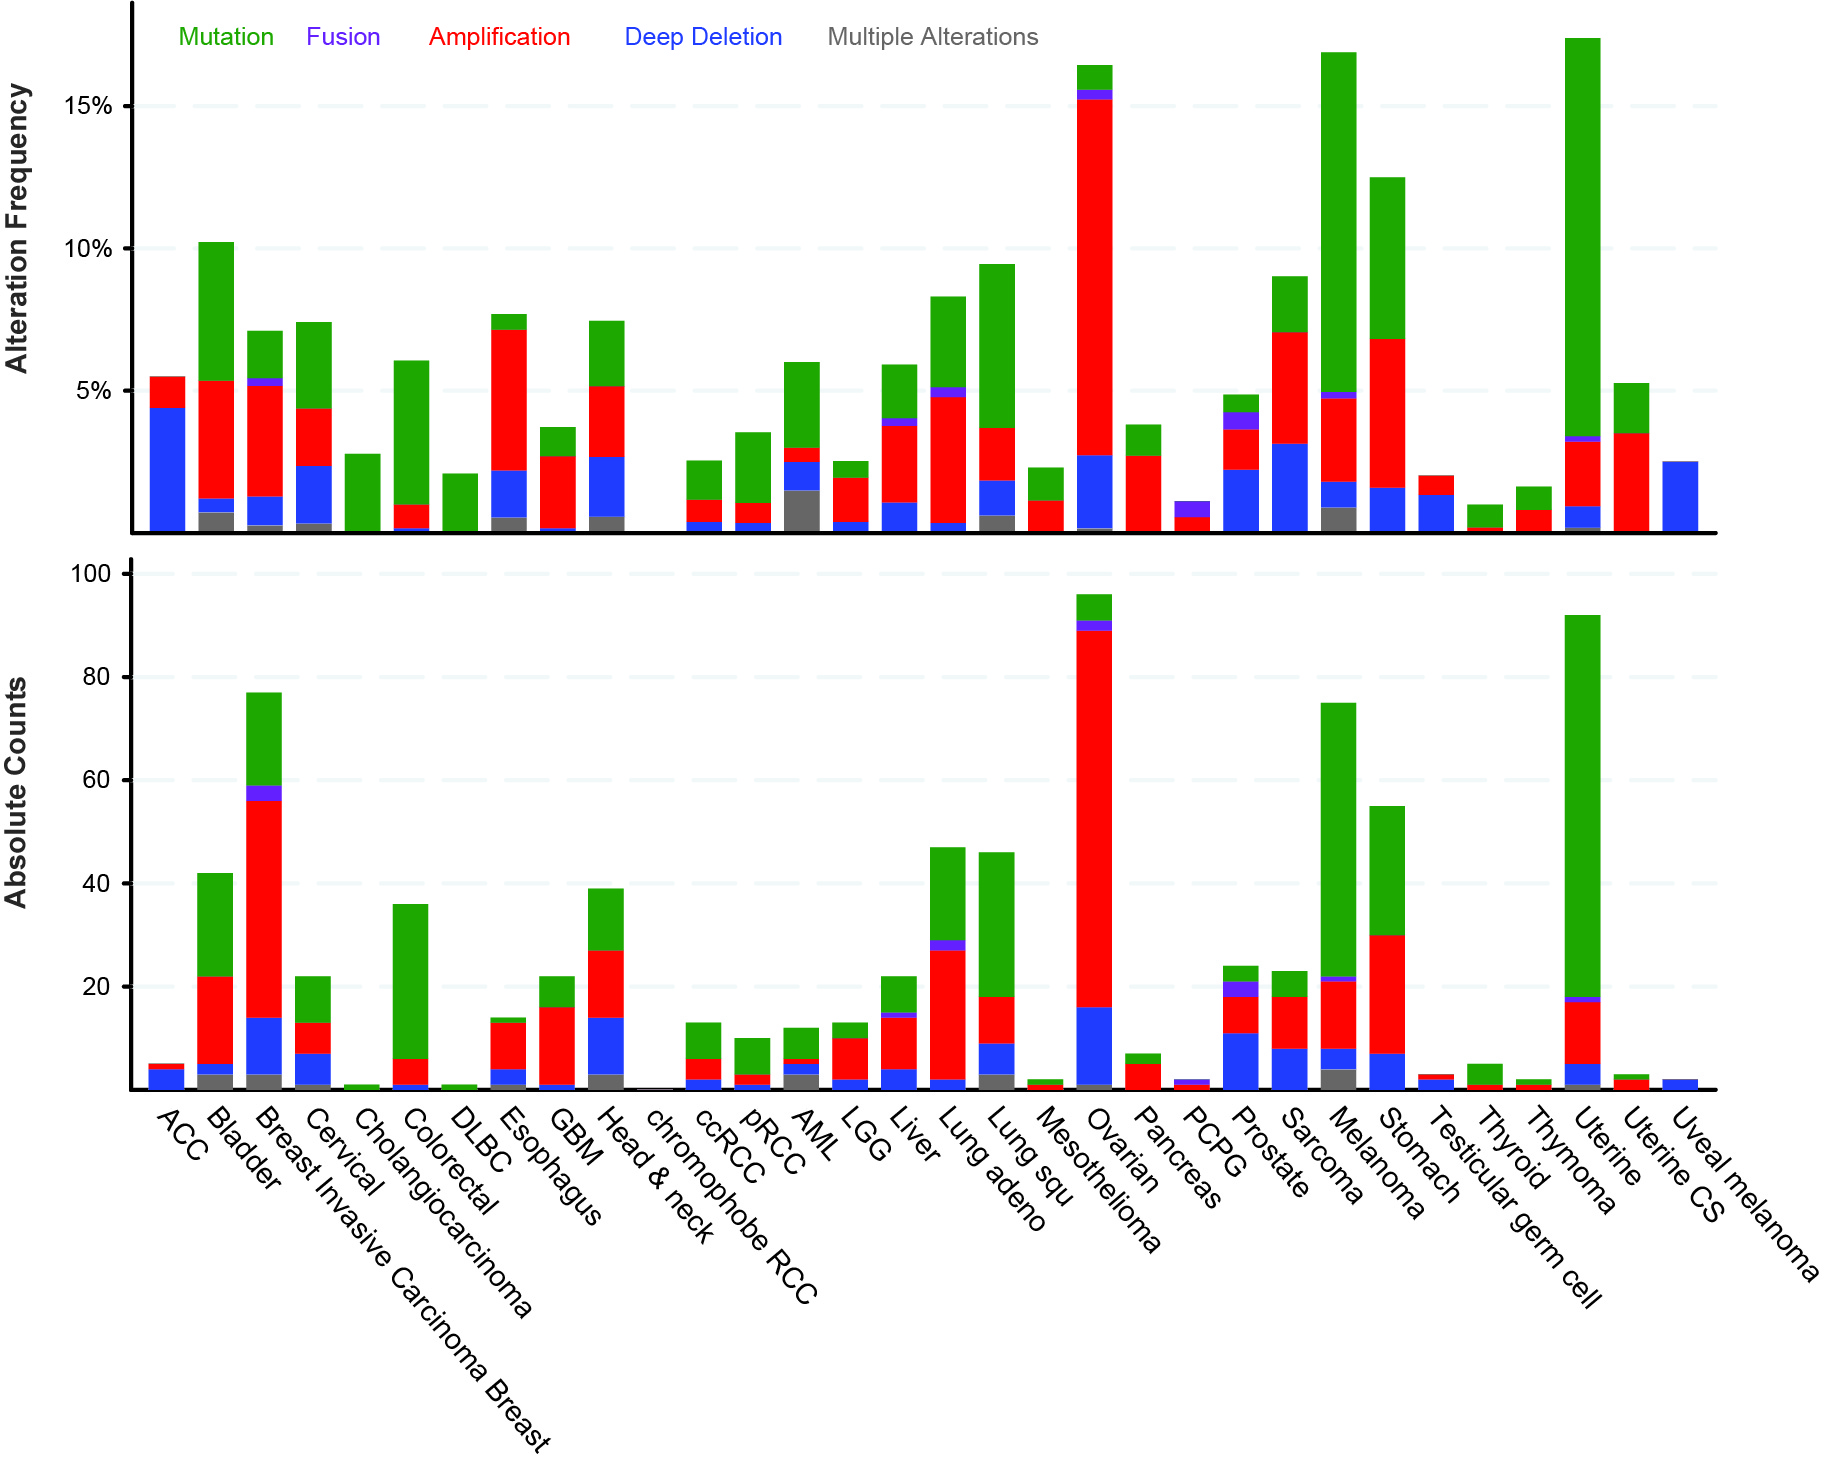
\includegraphics[width=155mm]{figures/aim3/FIG_number-of-samples.jpg}
\caption{
    \textbf{The frequency of alteration of PRC2 in different cancer types.}
    The frequency of alteration of PRC2 (top) and number of samples with altered PRC2 (bottom) in The Cancer Genome Atlas. Somatic mutations to \emph{EZH1}, \emph{EZH2}, \emph{EED}, and \emph{SUZ12} were included. \href{https://www.cbioportal.org/results/cancerTypesSummary?Action=Submit&RPPA_SCORE_THRESHOLD=2.0&Z_SCORE_THRESHOLD=2.0&cancer_study_list=laml_tcga_pan_can_atlas_2018\%2Cacc_tcga_pan_can_atlas_2018\%2Cblca_tcga_pan_can_atlas_2018\%2Clgg_tcga_pan_can_atlas_2018\%2Cbrca_tcga_pan_can_atlas_2018\%2Ccesc_tcga_pan_can_atlas_2018\%2Cchol_tcga_pan_can_atlas_2018\%2Ccoadread_tcga_pan_can_atlas_2018\%2Cdlbc_tcga_pan_can_atlas_2018\%2Cesca_tcga_pan_can_atlas_2018\%2Cgbm_tcga_pan_can_atlas_2018\%2Chnsc_tcga_pan_can_atlas_2018\%2Ckich_tcga_pan_can_atlas_2018\%2Ckirc_tcga_pan_can_atlas_2018\%2Ckirp_tcga_pan_can_atlas_2018\%2Clihc_tcga_pan_can_atlas_2018\%2Cluad_tcga_pan_can_atlas_2018\%2Clusc_tcga_pan_can_atlas_2018\%2Cmeso_tcga_pan_can_atlas_2018\%2Cov_tcga_pan_can_atlas_2018\%2Cpaad_tcga_pan_can_atlas_2018\%2Cpcpg_tcga_pan_can_atlas_2018\%2Cprad_tcga_pan_can_atlas_2018\%2Csarc_tcga_pan_can_atlas_2018\%2Cskcm_tcga_pan_can_atlas_2018\%2Cstad_tcga_pan_can_atlas_2018\%2Ctgct_tcga_pan_can_atlas_2018\%2Cthym_tcga_pan_can_atlas_2018\%2Cthca_tcga_pan_can_atlas_2018\%2Cucs_tcga_pan_can_atlas_2018\%2Cucec_tcga_pan_can_atlas_2018\%2Cuvm_tcga_pan_can_atlas_2018&case_set_id=all&data_priority=0&gene_list=EZH2\%252C\%2520EZH1\%252CEED\%252CSUZ12&geneset_list=\%20&profileFilter=0&tab_index=tab_visualize}{cBioPortal} was used to collect and visualize the data \cite{Cerami2012, Gao2013}.
}
\label{fig:num-samples-prc2}
\end{figure}

%%%%%%%%%%%%%%%%%%%%%%%%%%%%%%%%%%%%%%%%%%%
% Aim 3.1
%%%%%%%%%%%%%%%%%%%%%%%%%%%%%%%%%%%%%%%%%%%

\subsection*{Aim 3.1. Identify differences in mutations associated with dysregulated PRC2.}


\subsubsection*{Approach}

If the epigenetic state of a cell determines its susceptibility to different cancer driver genes, then we expect to find different genes mutated when PRC2 function is altered.
To this end, we will identify genes that are more or less frequently mutated in PRC2-dysfunctional tumors compared to those with normal PRC2. 
Of these genes, the properties of the known oncogenes, along with a functional enrichment analysis of the others, will describe the distinct changes induced by PRC2-mediated epigenetic changes.

We can identify more complex rearrangements of the cellular signaling structure by identifying new modules of comutating or mutually-exclusive genes in PRC2-dysfunctional tumors using existing computational methods \cite{Miller2011, Vandin2012, Ciriello2012, Jia2014, Zhang2014c, Ahmed2015, Kim2015, Leiserson2015, Babur2015, Leiserson2015b, Dao2017, Leiserson2016, Cho2016a, Reyna2018, Zhang2018e, Bokhari2020QuaDMutNetEx:Frequency.}.
Genes often comutate because the events cooperate in driving cancer or are mutually-exclusive because they are redundant or due to synthetic lethal \cite{Kaelin2005} or collateral lethal \cite{Muller2015} interactions.
Therefore, comutation or mutually exclusive interactions that are unique or lost in PRC2-mutant tumors would suggest that the epigenetic alterations have greatly influenced the signaling pathways.

It is known that chromatin structure plays a substantial role in the distribution of mutations along the chromosomes \cite{Schuster-Bockler2012, Polak2015, Gonzalez-Perez2019}.
Thus, the mutational patterns identified in the above analyses could be due, in part, to changes in their proximity in 3D-space or degree of chromosomal compaction elicited by altered PRC2 behaviour.
We will include this in the analysis by identifying "spatial comutation hotspots" \cite{Shi2016ChromatinGenes}, thus linking dysregulated PRC2-mediated chromatin organization to the increased rates of mutation or changes in comutation and mutually exclusive modules.
We will use the the epigenomic map created by the Roadmap Consortium \cite{Polak2015} as a reference for the normal chromatin state.

Overall, the analyses proposed above represent a comprehensive characterization of changes to cancer progression induced by aberrant PRC2 epigenetic regulation.


\subsubsection*{Pitfalls and alternative approaches}

As PRC2 is a protein complex with multiple subtypes thought to modify its recruitment and enzymatic function \cite{Wassef2017, Holoch2017, Kasinath2018, Laugesen2019a}, we expect different mutations of the subunits of PRC2 to have different impacts.
All of the genes encoding the core PRC2 subunits have known loss-of-function alterations and some, particularly \emph{EZH2}, have known gain-of-function alterations \cite{Comet2016MaintainingCancer.}.
Therefore, a careful survey of the RNA expression, copy number, and missense mutations to the genes comprising PRC2 will be conducted prior to the above analyses.

Since we want to prescribe altered rates of mutation to changes in PRC2 activity, knowing the timing of the events may be important.
The process of ordering mutations acquired during tumorigensis is best accomplished using single-cell analyses.
Thus, it may be possible to determine the timing of events in single-cell sequencing data of tumors where the component genes of PRC2 contained somatic mutations.
Further investigation is needed to fully understand if the analysis of single-cell genome sequencing is a viable means of determining the order of events identified in the previous analyses.



%%%%%%%%%%%%%%%%%%%%%%%%%%%%%%%%%%%%%%%%%%%
% Aim 3.2
%%%%%%%%%%%%%%%%%%%%%%%%%%%%%%%%%%%%%%%%%%%

\subsection*{Aim 3.2. Determine genetic dependencies associated with aberrant PRC2 function.}


\subsubsection*{Approach}

As dysregulated PRC2 alters the cellular signaling context of a tumor, we expect distinct dependencies on cellular processes to arise \cite{Kim2015SWI/SNF-mutantEZH2., Fillmore2015EZH2Inhibitors., Serresi2016PolycombCancer., Serresi2018Ezh2Vulnerabilities., Chen2018TargetingMedicine.}.
Thus, we will again utilize the Cancer Dependency Map Project's CRISPR-Cas9 knockout screen \cite{Tsherniak2017, Meyers2017} to identify genes that are differentially dependent in PRC2-mutant cancer cell lines.
As before, we will create a linear model for each gene that will use the RNA-expression of the gene, its mutational status, and the status of PRC2 to predict the effect of knocking-out the gene on the cell's proliferation.
We will also build models that include binary indicators for the common oncogenes and tumor suppressor genes found in each cancer type.
These models will be compared to estimate the importance of altered PRC2 activity on the dependency on each gene.
Further information from the genes found to have differential dependence per the activity of PRC2 will be gathered by finding which cellular processes are enriched in the results.

As we are interested in the potency of oncogenes in the presence of normal and altered PRC2 activity, we will also build specific models for the dependence of known oncogenes and those with increased or reduced rates of mutation in PRC2-mutant tumors (from Aim 3.1) that include an interaction term between the oncogene and PRC2 activity.
These terms will indicate whether there is an effect of a cell having a mutation to the oncogene and dysregulated PRC2 on the dependency of the cell on the oncogene.
Comparing these models to those without the interaction term will indicate if the interaction was important.


\subsubsection*{Pitfalls and alternative approaches}

An alternative approach to building a model for each individual gene as proposed above would be to build models for entire pathways or cellular functions instead.
This would recognize instances where the PRC2 dysregulation has caused the dependency on a group of genes to change, but where each cell line has different genes in the set that have altered dependency or the dependency is spread amongst multiple genes.
One foreseeable difficulty will be finding a single metric to summarise the dependency score for an entire pathway for each cell line.
One option would be to use Gene Set Variation Analysis \cite{Hanzelmann2013} or a related method \cite{Barbie2009, Lee2008InferringClassification., Tomfohr2005PathwayDecomposition., Jung2011ComparisonGenes.} to transform the gene level data into a pathway level enrichment score for each cell line.


% {\color{red} 
% Vinay's comments
% \begin{enumerate}
%     \item Why is "Rationale" incomplete? Are you filling this in?
%     \item For the spatial determinants -- you could also consider whether the co-mutated regions also exist within regions marked with specific chromatin modifications in normal tissue. Polak and colleagues checked for such context when inferring cell-of-origin. Additionally, if you are doing a co-mutation or mutational process study, you will need to control for local sequence composition
%     \item The rationale for why PRC2-activated would be mutated more in PRC2-mutant tumors is unclear, unless you already expect that open/closed chromatin in PRC2-mutant tumors have different mutational rates. 
% \end{enumerate}
% }